\chapter{Breve introduzione alla tecnologia iBeacon}
Gli iBeacon (anche detti BLE Beacon) sono dispositivi portatili, spesso alimentati a batteria, che integrano una radio Bluetooth. Il loro scopo è definire \textbf{regioni} di spazio delimitato dall'estensione del segnale che emettono in broadcast ripetutamente con una frequenza predefinita. Si rendono utili per \textit{micro-location system} in quanto offrendo una precisione molto senza forti ripercussioni sulla loro autonomia.

Spesso sono utilizzati come \textit{trigger} per App che integrano \textit{custom action}, reagendo alla prossimità, creando delle reazioni visibili sullo smartphone che utente appaiono come \textbf{interazioni col mondo fisico}.

La tecnologia chiave che permette agli iBeacon di funzionare è la \textbf{proximity specification BLE} (Bluetooth Low Energy), spesso indicata come \textbf{Bluetooth Smart}. BLE è un miglioramento della specifica Bluetooth che permette un consumo energetico ridotto che si ripercuote positivamente sull'autonomia dei dispositivi a batteria.

\begin{figure}[!ht]
	\centering
	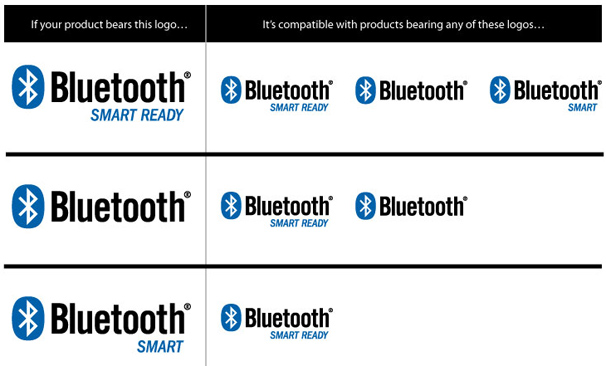
\includegraphics[scale=.25]{img/bt/BT.png}
	\caption{Compatibilità delle diverse tecnologie Bluetooth}
\end{figure}

Il limitato consumo energetico degli iBeacon si deve alla ridotta potenza di trasmissione di questa tecnologia che permette lunghi periodi di utilizzo (mesi o addirittura anni).

\section{Il protocollo iBeacon}
Il protocollo di comunicazione iBeacon è semplice e lineare. Si suddivide tra \textbf{broadcaster} (trasmettitore) e \textbf{receiver} (ricevitore). 

\subsection{Broadcaster}
Nella specifica Bluetooth, un iBeacon è per definizione un \textit{broadcaster}. I broadcaster trasmettono \textbf{advertising packet} periodici che contengono informazioni utilizzabili dai \textit{receiver}. 

\subsection{Receiver}
In questo protocollo i receiver non devono rispondere ai pacchetti che ricevono ed in generale i broadcaster non sono abilitati alla ricezione. La comunicazione degli advertising packet avviene sempre e solo attraverso una trasmissione unidirezionale.

\subsection{Advertising packet}
Essenzialmente gli advertising packet sono dispersi dai broadcaster nell'aria e i receiver possono scegliere se agire o no in base al loro contenuto.

La ricezione di un advertising packet da parte di un receiver provoca la creazione di un \textbf{advertisement event}. Per questo gli advertising packet e gli advertisement event genericamente sono denominati come \textbf{advertisement}. 

\begin{figure}[!ht]
	\centering
	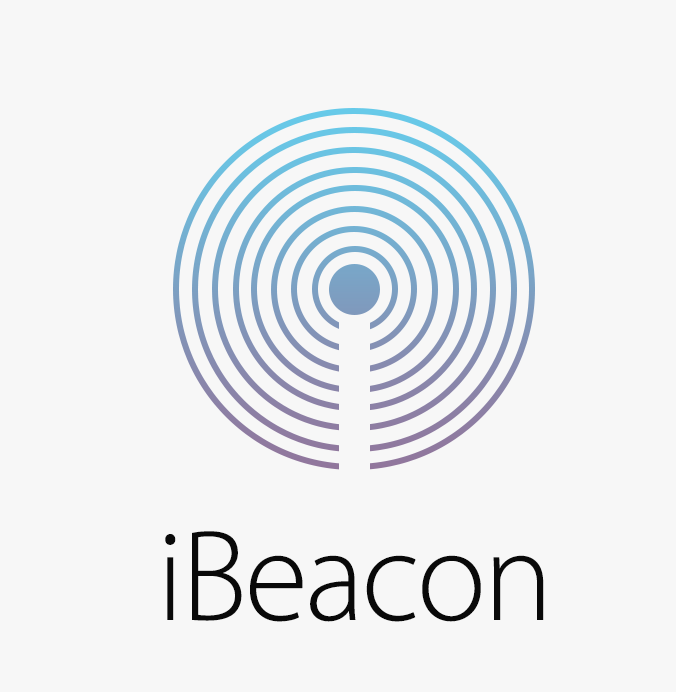
\includegraphics[scale=.20]{img/bt/ibeacon.png}
	\caption{Logo che identifica i dispositivi iBeacon}
\end{figure}

\section{Frame iBeacon}
Il formato del frame iBeacon è abbastanza semplice. Sono presenti solo un due parametri variabili che sono comunque sufficienti per supportare applicazioni complesse.

Le informazioni che un iBeacon emette si suddividono in tre identificativi:
\begin{itemize}
	\item Universal Unique Identifier
	\item Major number
	\item Minor number
\end{itemize}

\subsection{UUID (128 bits)}
L'UUID identifica univocamente la società di cui l'iBeacon fa parte. A differenza di altri protocolli di rete come 802.11, l'UUID non è gestito centralmente per evitare conflitti. Il protocollo Bluetooth presuppone che UUID siano unici.

L'UUID è il numero più facile da elaborare perché dovrebbe essere unico. Un sistema che supporta più brand name può utilizzare diversi UUID.

La maggior parte degli UUID sono creati da generatori di numeri casuali, spesso integrando l'ora corrente e un identificatore del generatore (ad esempio l'indirizzo MAC). Molte applicazioni per la configurazione di iBeacon commerciali hanno un pulsante per generare un UUID pseudocasuale.

\subsection{Major number (16 bits)}
Le specifiche Bluetooth e iBeacon non dispongono di una struttura per l'uso dei major o minor numers.

Il Major number viene utilizzato per identificare i Major groups di iBeacon di proprietà di un'unica entità. Nell'esempio della catena di negozi, il Major number tipicamente è utilizzato dai iBeacon che si trovano all'interno del negozio, identificando gruppi di proximity area in modo logico. Il campo a 16 bit permette di avere 65.000 possibilità.

\subsection{Minor number (16 bits)}
Il Minor number viene utilizzato per identificare il livello più basso della gerarchia all'interno di un insieme di iBeacon. Tornando all'esempio di una catena di negozi, il Minor number sarà utilizzato per i singoli iBeacon all'interno di una singola posizione del negozio, per esempio potrebbe identificare un prodotto esposto.

Il Minor number è una ulteriore suddivisione del raggruppamento definito dal Major number. I Minor number di solito si riferiscono ad una posizione geografica o POI all'interno di una posizione.

\section{RSSI - Received Signal Strength Indication}
La \textbf{proximity estimation} (stima di prossimità) dipende dal RSSI. RSSI non è trasmesso nel advertising packet, ma viene percepito dal receiver come il livello di potenza del segnale ricevuto.

\subsection{Advertising Interval}
Anche se le specifiche Bluetooth permettono di definire più \textit{advertising interval}, la specifica iBeacon fissa l'advertising interval a 100 ms.

L'impostazione dell'advertising interval è bilanciato in modo da preservare la vita della batteria, ma comunque essere abbastanza lungo per consentire ai servizi basati sugli iBeacon di funzionare.

\section{iBeacon Advertising Packet Contents}
Tutti i advertising packet hanno sempre la stessa lunghezza e sono composti da una serie di campi fissi. L'ultima parte del frame contiene informazioni specifiche del costruttore definito da Apple. È comunque possibile definire un formato pacchetto personalizzato in modo da migliorare le capacità di puntamento un iBeacon.

\begin{figure}[!ht]
	\centering
	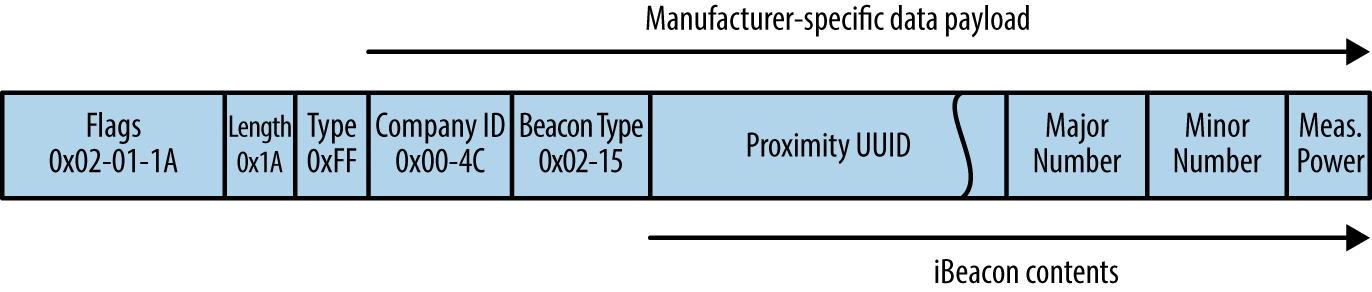
\includegraphics[scale=.25]{img/bt/iBeacon_advertising_packet_format.png}
	\caption{Formato di un iBeacon advertising packet format}
\end{figure}

\subsection{Measured power}
L'idea di \textbf{ranging} è implicita all'interno del protocollo iBeacon. Il \textit{ranging} indica la distanza tra il receiver e l'iBeacon analizzando le variazioni di potenza della trasmissione ricevuta. La distanza da un iBeacon viene stimata in base alla costante di calibrazione adeguata, misurando il tempo che un segnale impiega per poter essere ricevuto e la sua potenza.

Il \textit{Measured power} è un parametro impostato tenendo un receiver ad un metro dall'iBeacon e calcolando la media di RSSI. Questo campo contiene la potenza misurata come complemento a due. 

\paragraph{Esempio:} un valore di C5 indica che la potenza misurata a un metro è di -59 dBm.
\\\\Dati:
\begin{itemize}
	\item \texttt{0xC5\textsubscript{hex} = 197\textsubscript{dec}}
	\item \texttt{0x100\textsubscript{hex} = 256\textsubscript{dec}}
\end{itemize}
\begin{center}
	\texttt{(256 - 197) = -59 dBm}
\end{center}
